%% GCMM 2026 -- Special Session SS3 "Quantum-Enhanced Optimization and
%% Intelligent Control". OFFICIAL Springer Proceedings template (svproc),
%% as provided on the GCMM site for LNME/LNNS.
%% The class files svproc.cls + aliascnt.sty + remreset.sty are bundled
%% in this folder because svproc is NOT in TeXLive; on Overleaf start
%% from the official "ProcSci_TeX" template instead.
\documentclass{svproc}

\usepackage{graphicx}
\usepackage{amsmath,amssymb}
\usepackage{booktabs}
\usepackage{url}
% Springer proceedings: do NOT load hyperref in the final camera-ready.
\def\UrlFont{\rmfamily}

%% Blind-review toggle: \blindtrue = first (review) submission -- GCMM
%% requires a blind first version (no author names/affiliation/
%% acknowledgements); \blindfalse = camera-ready with full details.
\newif\ifblind
\blindtrue

\begin{document}
\mainmatter

\title{Gate-Model Quantum Neighborhood Search for the Permutation
       Flow Shop Problem via Fixed-Angle QAOA}
\titlerunning{Gate-Model Quantum Neighborhood Search for the PFSP}

\ifblind
  \author{}
  \authorrunning{}
  \institute{}
\else
  \author{Remigiusz Wojew\'{o}dzki \and Wojciech Bo\.{z}ejko}
  \authorrunning{R. Wojew\'{o}dzki and W. Bo\.{z}ejko}
  % GCMM: corresponding author only, corporate (institutional) e-mail only.
  \institute{Wroc\l{}aw University of Science and Technology, Faculty of
    Information and Communication Technology, Department of Control and
    Quantum Computing, Wroc\l{}aw, Poland,\\
    \email{wojciech.bozejko@pwr.edu.pl}}
\fi

\maketitle

\begin{abstract}
The permutation flow shop problem (PFSP) is a canonical NP-hard
scheduling problem whose local-search solvers spend most of their
effort evaluating neighborhood moves. Recent work has offloaded this
evaluation to quantum annealers by casting neighborhoods as QUBO
problems, yet the gate-model paradigm -- despite its flexible
connectivity -- remains largely unexplored for scheduling. This paper
introduces a gate-model framework that evaluates PFSP neighborhoods with
the Quantum Approximate Optimization Algorithm (QAOA) embedded in
classical Iterated Local Search and Simulated Annealing metaheuristics,
giving a hybrid quantum--classical scheme for quantum-enhanced
scheduling. We reuse the swap-selection QUBO encoding from the annealing
line, so a single problem matrix drives either an annealer or a QAOA
circuit, and we adopt a fixed-angle QAOA whose variational angles are
pre-optimized offline; on hardware each move then costs a single circuit
execution, keeping the method viable under NISQ constraints. We
formulate all four neighborhood structures (Adjacent, Fibonacci,
Dynasearch, Motzkin) and analyze how their conflict-graph density
governs circuit depth once the QUBO is compiled onto heavy-hex
superconducting hardware. We show that depth assumes the role that
embedding capacity plays on annealers, producing the same feasibility
ordering for a different, compilation-grounded reason, and we discuss
windowed decomposition as a means of taming dense neighborhoods. The
paper sets out the evaluation methodology and the open challenges on the
path to on-hardware execution.
\keywords{combinatorial optimization, QUBO, metaheuristics, simulated
  annealing, circuit compilation on heavy-hex hardware, NISQ}
\end{abstract}

% =====================================================================
\section{Introduction}
\label{sec:intro}
% PFSP + neighborhood-based metaheuristics; move evaluation is the
% bottleneck. Quantum line so far: annealing only (D-Wave); gate model
% unexplored for scheduling. Contribution: gate-model QAOA framework,
% fixed-angle, swap-selection QUBO reused, 4 neighborhoods, depth =
% gate-model analog of the annealer embedding limit.

% =====================================================================
\section{Literature Review}
\label{sec:related}
% VLSN / PFSP neighborhoods; QUBO/Ising formulations; QAOA and
% fixed-angle QAOA; quantum-enhanced scheduling (annealing companion).

% =====================================================================
\section{Research Methodology}
\label{sec:method}

Our framework leaves the classical metaheuristic untouched and replaces
only the neighborhood-evaluation oracle with a gate-model quantum
subroutine. Every move evaluation is cast as a QUBO instance, mapped to
an Ising Hamiltonian, and solved approximately by a fixed-angle QAOA
circuit~\cite{farhi2014qaoa}. This mirrors the annealing line of
work~\cite{wojewodzki2026bpasts,wojewodzki2026windowed}: a single
swap-selection QUBO drives either a quantum annealer or a gate-model
QAOA circuit, so only the solver backend changes and the two paradigms
are compared on identical instances. The quantum subroutine is embedded,
unchanged, in the same Iterated Local Search and Simulated Annealing
hosts used by the annealing line.

\subsection{Swap-selection QUBO encoding}
\label{subsec:qubo}
We reuse the swap-selection encoding of the annealing
line~\cite{wojewodzki2026bpasts}. A binary variable $x_k=1$ indicates
that swap candidate $k$ is applied to the current permutation. Selecting
a subset of compatible swaps is written as the minimization of a
quadratic form
\begin{equation}
  \min_{\mathbf{x}\in\{0,1\}^{K}}\
  \mathbf{x}^{\mathsf T} Q\,\mathbf{x},
  \label{eq:qubo}
\end{equation}
where the diagonal entry $Q_{kk}=\delta_k$ is the makespan change induced
by swap $k$, evaluated in $O(1)$ time through the Head--Tail
decomposition, and the off-diagonal entry $Q_{kl}=\lambda$ penalizes
every conflicting pair of swaps. The penalty
\begin{equation}
  \lambda \;=\; \sum_{k=1}^{K}\lvert\delta_k\rvert \;+\; 1
  \label{eq:penalty}
\end{equation}
dominates the objective, so any solution that selects two conflicting
swaps is more expensive than any feasible one. The pattern of penalized
pairs is the fingerprint of the neighborhood
(Section~\ref{subsec:neigh}). Crucially, $Q$ in~\eqref{eq:qubo} is the
same matrix submitted to the quantum annealer in the companion
work~\cite{wojewodzki2026windowed}; only the solver that follows differs.

\subsection{From the QUBO to a QAOA circuit}
\label{subsec:circuit}
The change of variables $Z_k=2x_k-1$, i.e.\ $x_k=(1+Z_k)/2$, turns the
QUBO~\eqref{eq:qubo} into an Ising cost
Hamiltonian~\cite{lucas2014ising}
\begin{equation}
  H_C \;=\; \sum_{i} h_i Z_i \;+\; \sum_{i<j} J_{ij} Z_i Z_j
  \;+\; \mathrm{const},
  \label{eq:ising}
\end{equation}
whose linear fields $h_i$ and couplings $J_{ij}$ are obtained directly
from the entries of $Q$. A depth-$p$ QAOA prepares the parameterized
state
\begin{equation}
  \lvert\gamma,\beta\rangle \;=\;
  \Bigl(\textstyle\prod_{l=1}^{p}
        e^{-i\beta_l H_M}\,e^{-i\gamma_l H_C}\Bigr)
  \lvert +\rangle^{\otimes K},
  \qquad H_M=\sum_i X_i,
  \label{eq:qaoa}
\end{equation}
with the transverse-field mixer $H_M$. For $p=1$ each layer compiles to
elementary gates. An initial layer of Hadamard gates places the register
in an equal superposition over all move selections. The cost evolution
$e^{-i\gamma H_C}$ is realized as a single-qubit rotation
$R_Z(2\gamma h_i)$ on every variable together with a two-qubit rotation
$R_{ZZ}(2\gamma J_{ij})$ on every coupled pair, and the mixer
$e^{-i\beta H_M}$ as a rotation $R_X(2\beta)$ on every qubit. Sampling
the circuit and taking the most frequent bitstring yields the selected
swap set, that is, the chosen neighborhood move. Figure~\ref{fig:qaoa_fib}
shows the resulting $p=1$ circuit for a small Fibonacci instance. The set
of $R_{ZZ}$ gates is exactly the edge set of the conflict graph of $Q$,
so the neighborhood structure alone determines the two-qubit layer of the
circuit.

\begin{figure}[t]
\centering
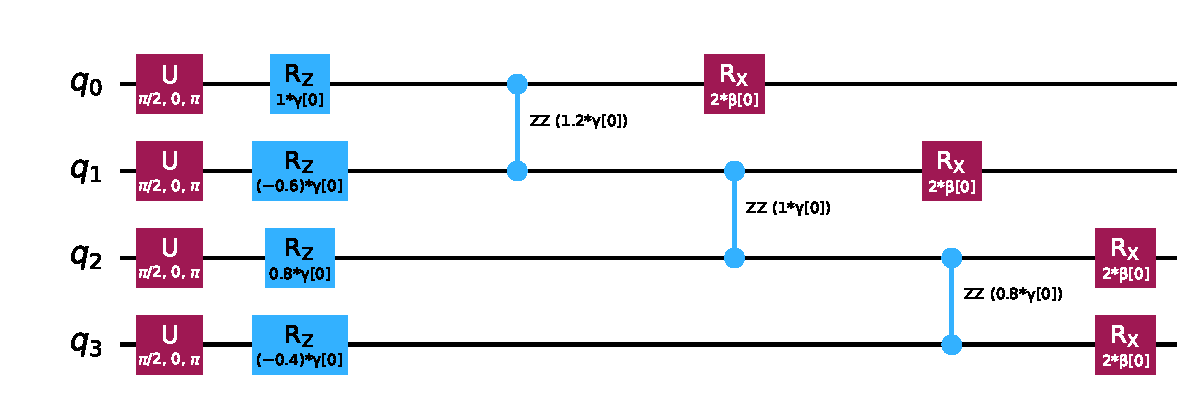
\includegraphics[width=\textwidth]{figures/qaoa_circuit_fibonacci}
\caption{QAOA circuit ($p=1$) for a four-variable Fibonacci
  neighborhood. Left to right: a Hadamard preparation layer, the
  single-qubit $R_Z$ cost-bias rotations (angles $\propto\delta_k$), the
  nearest-neighbor $R_{ZZ}$ couplings that encode the tridiagonal
  conflict graph, and the $R_X$ mixer.}
\label{fig:qaoa_fib}
\end{figure}

\subsection{Fixed-angle QAOA with offline angle optimization}
\label{subsec:fixed}
Variational QAOA re-optimizes the angles $(\gamma,\beta)$ for every
instance, spending tens to hundreds of circuit executions before a single
move is chosen. Under NISQ noise and a tight quantum-runtime budget---the
IBM Open plan grants roughly ten minutes of QPU time per twenty-eight-day
window---this is not viable inside a metaheuristic that evaluates
thousands of moves. We therefore fix the angles per neighborhood type and
obtain them offline, once. For each of the four neighborhoods a single
angle pair $(\gamma^\star,\beta^\star)$ is optimized on a classical
statevector simulator (Qiskit Aer) by minimizing the expected cost
\begin{equation}
  (\gamma^\star,\beta^\star)
  \;=\; \arg\min_{\gamma,\beta}\
  \langle\gamma,\beta\lvert H_C\rvert\gamma,\beta\rangle,
  \label{eq:angleopt}
\end{equation}
averaged over a small training set of representative QUBO instances of
that neighborhood. The angles are then frozen and reused for every move
of that neighborhood at run time, so the offline cost is amortized over
the whole search and the online cost per move stays at a single circuit
execution. This strategy relies on angle transferability: for a fixed
neighborhood the optimal $p=1$ angles are near-constant across instances,
a property we verify on the simulator before freezing. As a
training-free baseline we also report the instance-independent $p=1$
angles given by the fixed-angle conjectures of Wurtz and
Love~\cite{wurtz2021fixed}. On hardware each move therefore costs one
circuit execution, the direct gate-model analog of the annealer's single
call per move, which is the basis for a fair wall-clock comparison. We
work at $p=1$, the depth that current NISQ hardware supports reliably,
and consider $p=2$ only where the simulator shows a clear gain.

\subsection{Neighborhoods and their conflict graphs}
\label{subsec:neigh}
All four neighborhoods reuse their annealing
QUBOs~\cite{wojewodzki2026bpasts,wojewodzki2026soco} and differ only in
the coupling pattern of the $R_{ZZ}$ layer in~\eqref{eq:qaoa}, that is,
in the topology of the conflict graph. The Adjacent neighborhood selects
one of the $n-1$ adjacent transpositions under a one-hot constraint, so
every pair of variables conflicts and its conflict graph is complete. The
Fibonacci neighborhood penalizes only consecutive overlapping swaps and
so yields a tridiagonal chain, the sparsest of the four. The Dynasearch
and Motzkin neighborhoods both act on endpoint-swap intervals but apply
different conflict rules: Dynasearch penalizes every pair of overlapping
intervals, nested ones included, whereas Motzkin admits nested intervals
and penalizes only crossings and shared endpoints. Motzkin's conflict
graph is therefore a subgraph of Dynasearch's and is strictly sparser,
which is precisely the property that motivates the Motzkin
neighborhood~\cite{wojewodzki2026soco}. The Adjacent and Dynasearch
graphs are dense and compile to the deepest circuits, while the Fibonacci
and Motzkin graphs are sparse and stay shallow.
Figure~\ref{fig:neigh_circuits} shows example $p=1$ circuits for the
Adjacent, Dynasearch, and Motzkin neighborhoods; the Fibonacci circuit is
the one in Fig.~\ref{fig:qaoa_fib}. Each $R_{ZZ}$ gate corresponds to one
edge of the conflict graph, so the two-qubit gate count is read directly
off the graph.

\begin{figure}[p]
\centering
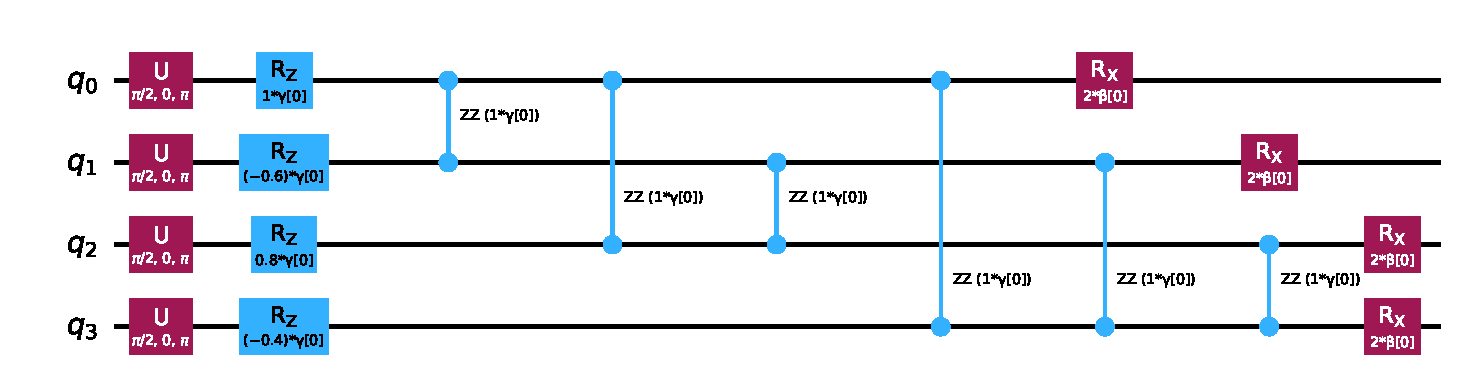
\includegraphics[width=\textwidth]{figures/qaoa_adjacent}\\[0.4ex]
{\footnotesize (a) Adjacent: complete conflict graph (dense)}\\[2.2ex]
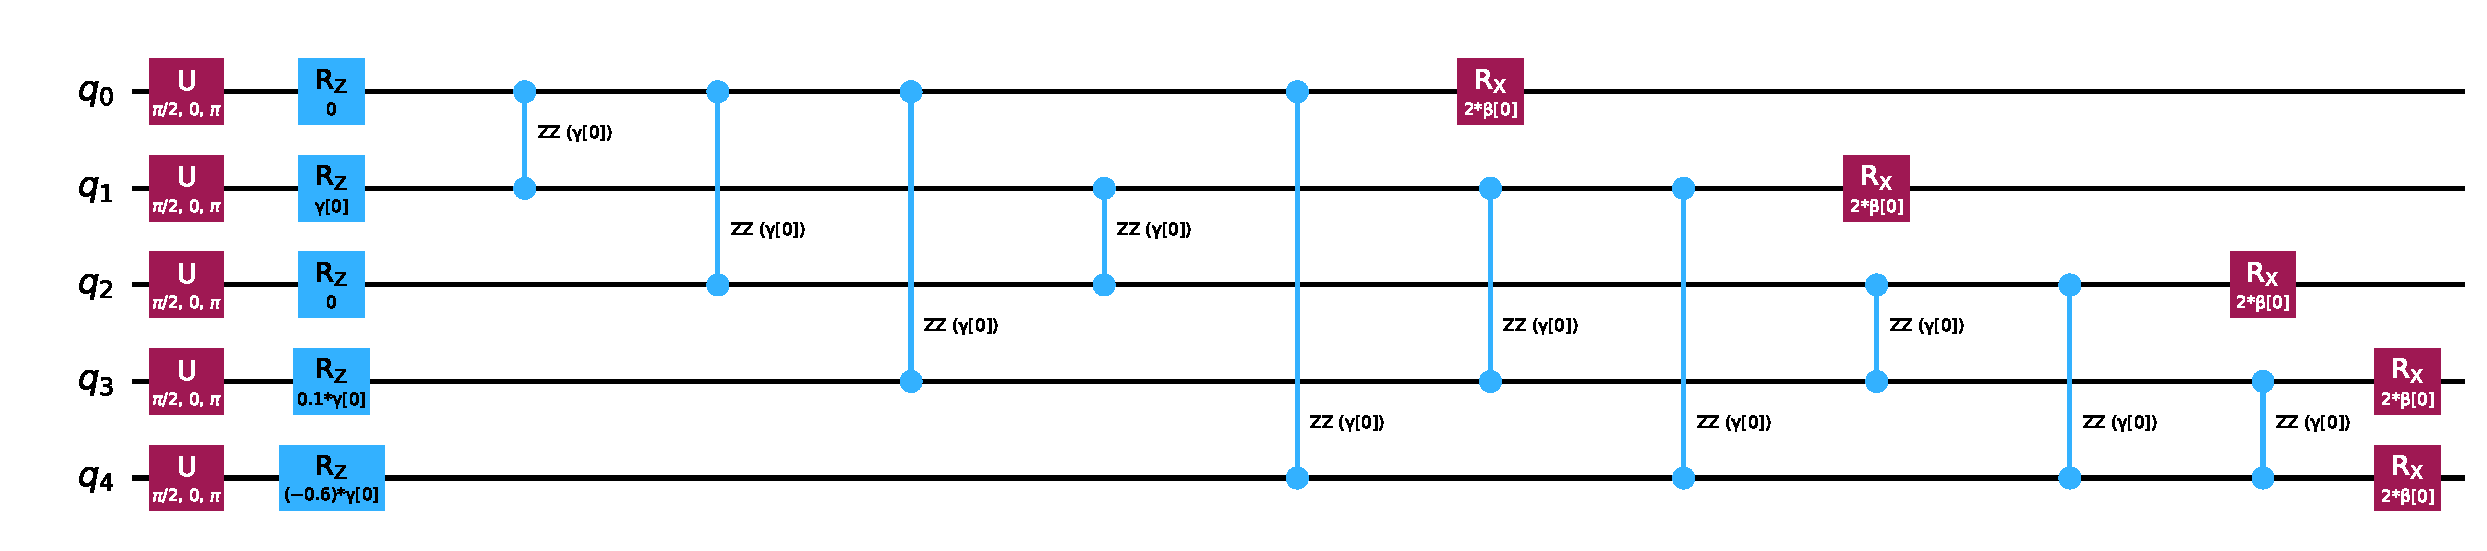
\includegraphics[width=\textwidth]{figures/qaoa_dynasearch}\\[0.4ex]
{\footnotesize (b) Dynasearch: all interval overlaps penalized (dense)}\\[2.2ex]
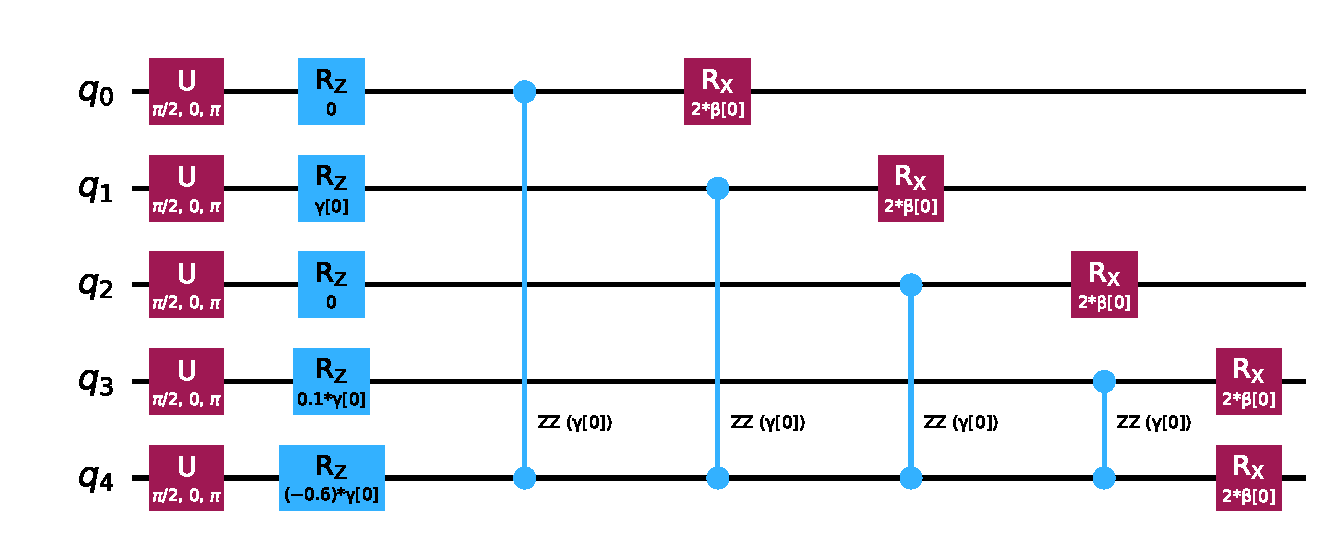
\includegraphics[width=\textwidth]{figures/qaoa_motzkin}\\[0.4ex]
{\footnotesize (c) Motzkin: nesting admitted, only crossings penalized (sparse)}
\caption{Example QAOA cost-and-mixer layers ($p=1$) for the Adjacent,
  Dynasearch, and Motzkin neighborhoods; the Fibonacci circuit is shown
  in Fig.~\ref{fig:qaoa_fib}. Each $R_{ZZ}$ gate corresponds to one edge
  of the conflict graph of the QUBO.}
\label{fig:neigh_circuits}
\end{figure}

\subsection{Compilation on heavy-hex hardware}
\label{subsec:depth}
On IBM Heron the physical qubit graph is heavy-hex, so each $R_{ZZ}$ gate
requires its two qubits to be physically adjacent. Non-adjacent pairs are
routed by inserting SWAP networks, which deepen the circuit and inject
additional noise. Circuit depth after transpilation therefore plays the
role that embedding capacity plays on the annealer: a dense conflict
graph such as Adjacent's or Dynasearch's compiles to a deep, noisy
circuit, whereas a sparse one such as Fibonacci's or Motzkin's stays
shallow. The resulting feasibility
ordering of the four neighborhoods matches the one observed on the
annealer, but for a different, compilation-grounded reason. For the dense
neighborhoods we reuse the windowed decomposition of the annealing
line~\cite{wojewodzki2026windowed}: solving the QUBO on small overlapping
windows keeps each per-window circuit shallow enough to run within the
coherence budget of the hardware.

\subsection{Hardware and software}
\label{subsec:hw}
The circuits target the IBM Heron~r2 processor \texttt{ibm\_fez} (156
qubits, heavy-hex coupling map, native gate set CZ, RZ, SX, X), accessed
through Qiskit Runtime (\texttt{qiskit}~2.5.1 with
\texttt{qiskit-ibm-runtime}). Development follows a simulator-first
protocol: we validate each neighborhood on the statevector Aer simulator,
then on a noisy fake-Heron backend, and only then commit a single
confirmatory run on \texttt{ibm\_fez}, so that scarce QPU time is spent
only on the final measurement rather than on debugging or angle tuning.

% =====================================================================
\section{Results and Discussion}
\label{sec:results}
% Evaluation methodology; per-neighborhood circuit depth / feasibility
% ordering; move-selection behavior; open challenges toward on-hardware
% runs. (Scope: framework + analysis; hard experiments may follow in an
% extended version.)

% =====================================================================
\section{Conclusions}
\label{sec:conclusions}
% Portable hybrid quantum-classical local-search scheme bridging the
% annealing and gate paradigms; depth-as-embedding-limit result;
% Motzkin nesting hypothesis; path to on-hardware execution.

% =====================================================================
\ifblind\else
\subsubsection{Acknowledgements.}
% Funding / D-Wave & IBM Quantum access acknowledgements; AI-assistance
% disclosure per venue policy. (Removed in the blind version.)
\fi

% =====================================================================
\begin{thebibliography}{9}

\bibitem{farhi2014qaoa}
Farhi, E., Goldstone, J., Gutmann, S.: A Quantum Approximate
Optimization Algorithm. arXiv:1411.4028 (2014)

\bibitem{lucas2014ising}
Lucas, A.: Ising formulations of many NP problems. Front. Phys.
\textbf{2}, 5 (2014)

\bibitem{wurtz2021fixed}
Wurtz, J., Love, P.: Fixed-angle conjectures for the quantum
approximate optimization algorithm on regular MaxCut graphs.
Phys. Rev. A \textbf{103}, 042612 (2021)

\bibitem{wojewodzki2026soco}
Wojew\'{o}dzki, R., Bo\.{z}ejko, W.: Motzkin Neighborhood Evaluation in
Iterated Local Search and Simulated Annealing for the Permutational
Flow Shop Problem. In: SOCO 2026, CCIS, vol.\ 3046, pp.\ 144--155.
Springer (2026). \url{https://doi.org/10.1007/978-3-032-29254-4_12}

\bibitem{wojewodzki2026bpasts}
Wojew\'{o}dzki, R., Bo\.{z}ejko, W.: Classical and Quantum Neighborhoods
Evaluation in Iterated Local Search and Simulated Annealing for the
Permutation Flow Shop Problem. Bull. Pol. Acad. Sci. Tech. Sci.
(under review, 2026)

\bibitem{wojewodzki2026windowed}
Wojew\'{o}dzki, R., Bo\.{z}ejko, W.: Scalable Quantum Neighborhood Search
for the Permutation Flow Shop Problem via Windowed QUBO Decomposition.
Comput. Oper. Res. (in preparation, 2026)

\bibitem{taillard1993}
Taillard, E.: Benchmarks for basic scheduling problems. Eur. J. Oper.
Res. \textbf{64}(2), 278--285 (1993)

% TODO: rozszerzyć -- QAOA transferability of angles, heavy-hex
% compilation/transpilation, PFSP tabu/VLSN.

\end{thebibliography}

\end{document}
